\section{Examples}\label{sec:examples}


The size of boundary matrix is critical parameter of LAR-SURF method. To determine optimal size of boundary matrix the experiment on artifical data was performed (Fig.  \ref{fig:bm_size_tesla}). Size of experimental data is set to $512\times512\times512$ and it is derived from typical size of Computed Tomography medical images. Computation is done on Tesla DGX-1 machine

\begin{figure}
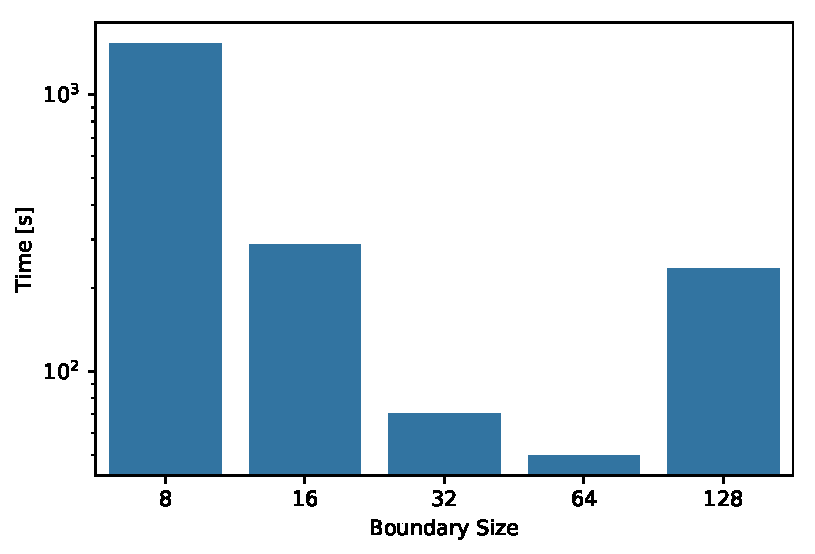
\includegraphics[width=0.99\textwidth]{figs/bm_size_tesla.pdf} 
%\includegraphics[scale=1]{input/ircad_comparison.pdf} 
\caption{Time requirements of LAR-SURF filter used on artifical with different size of boundary matrix}
\label{fig:bm_size_tesla}
\end{figure}

The 
For an experiments the we used the dataset Ircad1b. 

\begin{table}
\begin{tabular}{rrrrrr}
\toprule
 ID &  z-resolution [mm] &  xy-resolution [mm] &  obj. voxels &  size xy &  size z \\
\midrule
  1 &               1.60 &            0.570000 &      2865131 &      512 &     129 \\
  2 &               1.60 &            0.782000 &      1648024 &      512 &     172 \\
  3 &               1.25 &            0.625000 &      2375079 &      512 &     200 \\
  4 &               2.00 &            0.742188 &      1132427 &      512 &      91 \\
  5 &               1.60 &            0.782000 &      2124505 &      512 &     139 \\
  6 &               1.60 &            0.782000 &      1828493 &      512 &     135 \\
  7 &               1.60 &            0.782000 &      1461944 &      512 &     151 \\
  8 &               1.60 &            0.561000 &      3215090 &      512 &     124 \\
  9 &               2.00 &            0.873047 &      1265420 &      512 &     111 \\
 10 &               1.60 &            0.736000 &      1871804 &      512 &     122 \\
 11 &               1.60 &            0.720000 &      1692716 &      512 &     132 \\
 12 &               1.00 &            0.679688 &      3341433 &      512 &     260 \\
 13 &               1.60 &            0.671000 &      2063109 &      512 &     122 \\
 14 &               1.60 &            0.720000 &      1633641 &      512 &     113 \\
 15 &               1.60 &            0.782000 &      1389572 &      512 &     125 \\
 16 &               1.60 &            0.698000 &      2717185 &      512 &     155 \\
 17 &               1.60 &            0.743000 &      2106497 &      512 &     119 \\
 18 &               2.50 &            0.742188 &      1220564 &      512 &      74 \\
 19 &               4.00 &            0.703125 &       583208 &      512 &     124 \\
 20 &               2.00 &            0.808594 &      1359697 &      512 &     225 \\
\bottomrule
\end{tabular}

\end{table}
\begin{table}
\begin{tabular}{lrrrrr}
\toprule
{} &  z-resolution [mm] &  xy-resolution [mm] &   obj. voxels &  size xy &      size z \\
\midrule
% count &           20.00000 &           20.000000 &  2.000000e+01 &     20.0 &   20.000000 \\
min   &            1.00000 &            0.561000 &  5.832080e+05 &    512.0 &   74.000000 \\
mean  &            1.77750 &            0.725141 &  1.894777e+06 &    512.0 &  141.150000 \\
50\%   &            1.60000 &            0.739094 &  1.760604e+06 &    512.0 &  127.000000 \\
% std   &            0.60273 &            0.077233 &  7.206126e+05 &      0.0 &   44.088756 \\
% 25\%   &            1.60000 &            0.693422 &  1.382103e+06 &    512.0 &  121.250000 \\
% 75\%   &            1.70000 &            0.782000 &  2.187148e+06 &    512.0 &  152.000000 \\
max   &            4.00000 &            0.873047 &  3.341433e+06 &    512.0 &  260.000000 \\
\bottomrule
\end{tabular}

\end{table}


We performed experiment on Ircad dataset to compare time requirements and used t-test  check the  Based on $\alpha=0.99$ the with the $p=\num[]{8.735e-24}$ , 
$s=\num[]{-16.67}$


\begin{figure}
\includegraphics[width=0.99\textwidth]{figs/ircad_comparison.pdf} 
%\includegraphics[scale=1]{input/ircad_comparison.pdf} 
\caption{Time requirements of LAR-SURF filter and Marching Cubes on Ircad dataset. Error bars shows the 95\% confidence interval}
\label{fig:ircad_comparison}
\end{figure}